\section{Task Definition}
\label{sec:task}
%The temporally ordered user interactions lead to the streaming nature of session data. Therefore it's natural and realistic to formulate the news recommendation task as a session-based recommendation task to predict next-item. 
\tabref{tb:note} summarizes some basic symbols and notations used later, 
and in later sections, for brevity, we ignore $u$ superscript when discussing the information
for any user.
To explain further, the articles that appear in user $u$'s impression list are denoted as set $Imp_u$. An impression list is the articles in the vicinity of the articles
being clicked, which may have left an impression on the user.

Assume that $S_u$'s length is $T$, and can be represented as \[S_u: (n_1^u,c_1^u,t_1^u)\rightarrow(n_2^u,c_2^u,t_2^u)\rightarrow...\rightarrow(n_i^u,c_i^u,t_i^u),\] 
In the training phase, the recommendation system aims to model the 
user feedback sequence as vector $\mathbf{x_s}$, 
maximizing the similarity between
the vector of predicted next-article ($n_{i+1}^u$) and $\mathbf{x_s}$. 
While in the test phase, 
given interaction sequence $S_u$ as input, 
we produce a ranking list $R$ with the probability that the target user $u$ is likely to click next from high to low. 
Typically a recommender needs to recommend more
than one item for a user, thus the top-k items in $R$ are recommended.
Noted that each user $u$ only appears once, 
which means training set and test set don't share the same users. 

\begin{table}
    \caption{Symbols notations and descriptions}
    \begin{tabular}{cc}
    \toprule
    $S_u$ & A session produced by an anonymous user $u$.\\
    $i$ & $i\in [1,T]$ indexs articles in $S_u$.\\
    $n_i^u$ & The id of $i$-th article clicked by $u$.\\
    $c_i^u$ & The Content representation of $n_i^u$ \\
    $t_i^u$ & The active time that $u$ stays in $n_i^u$. \\
    $Imp_u$ & Set of articles that appear in $u$'s impression.\\
    $\mathbf{x}_i$ & The embedding vector of $n_i^u$.\\
    $\mathbf{x_s}$ & The session vector of $S_u$ encoded by model.\\
    $N$ & The total number of articles.\\
    $j$ & $j\in [1,N]$ indexs the article in total articles.\\
    $\hat{y_j}^u$ & The score of $n_j$ being clicked by $u$ next.\\
    $R$ & Ranking list generated according to $\hat{y_j}^u$.\\
    $Ne_u$ & The set of negative samples.\\
    \bottomrule
    \end{tabular}
    \label{tb:note}
\end{table}
% The whole procedure is depicted in \figref{fig:task}.

% \begin{figure}[th]
%     \centering
%     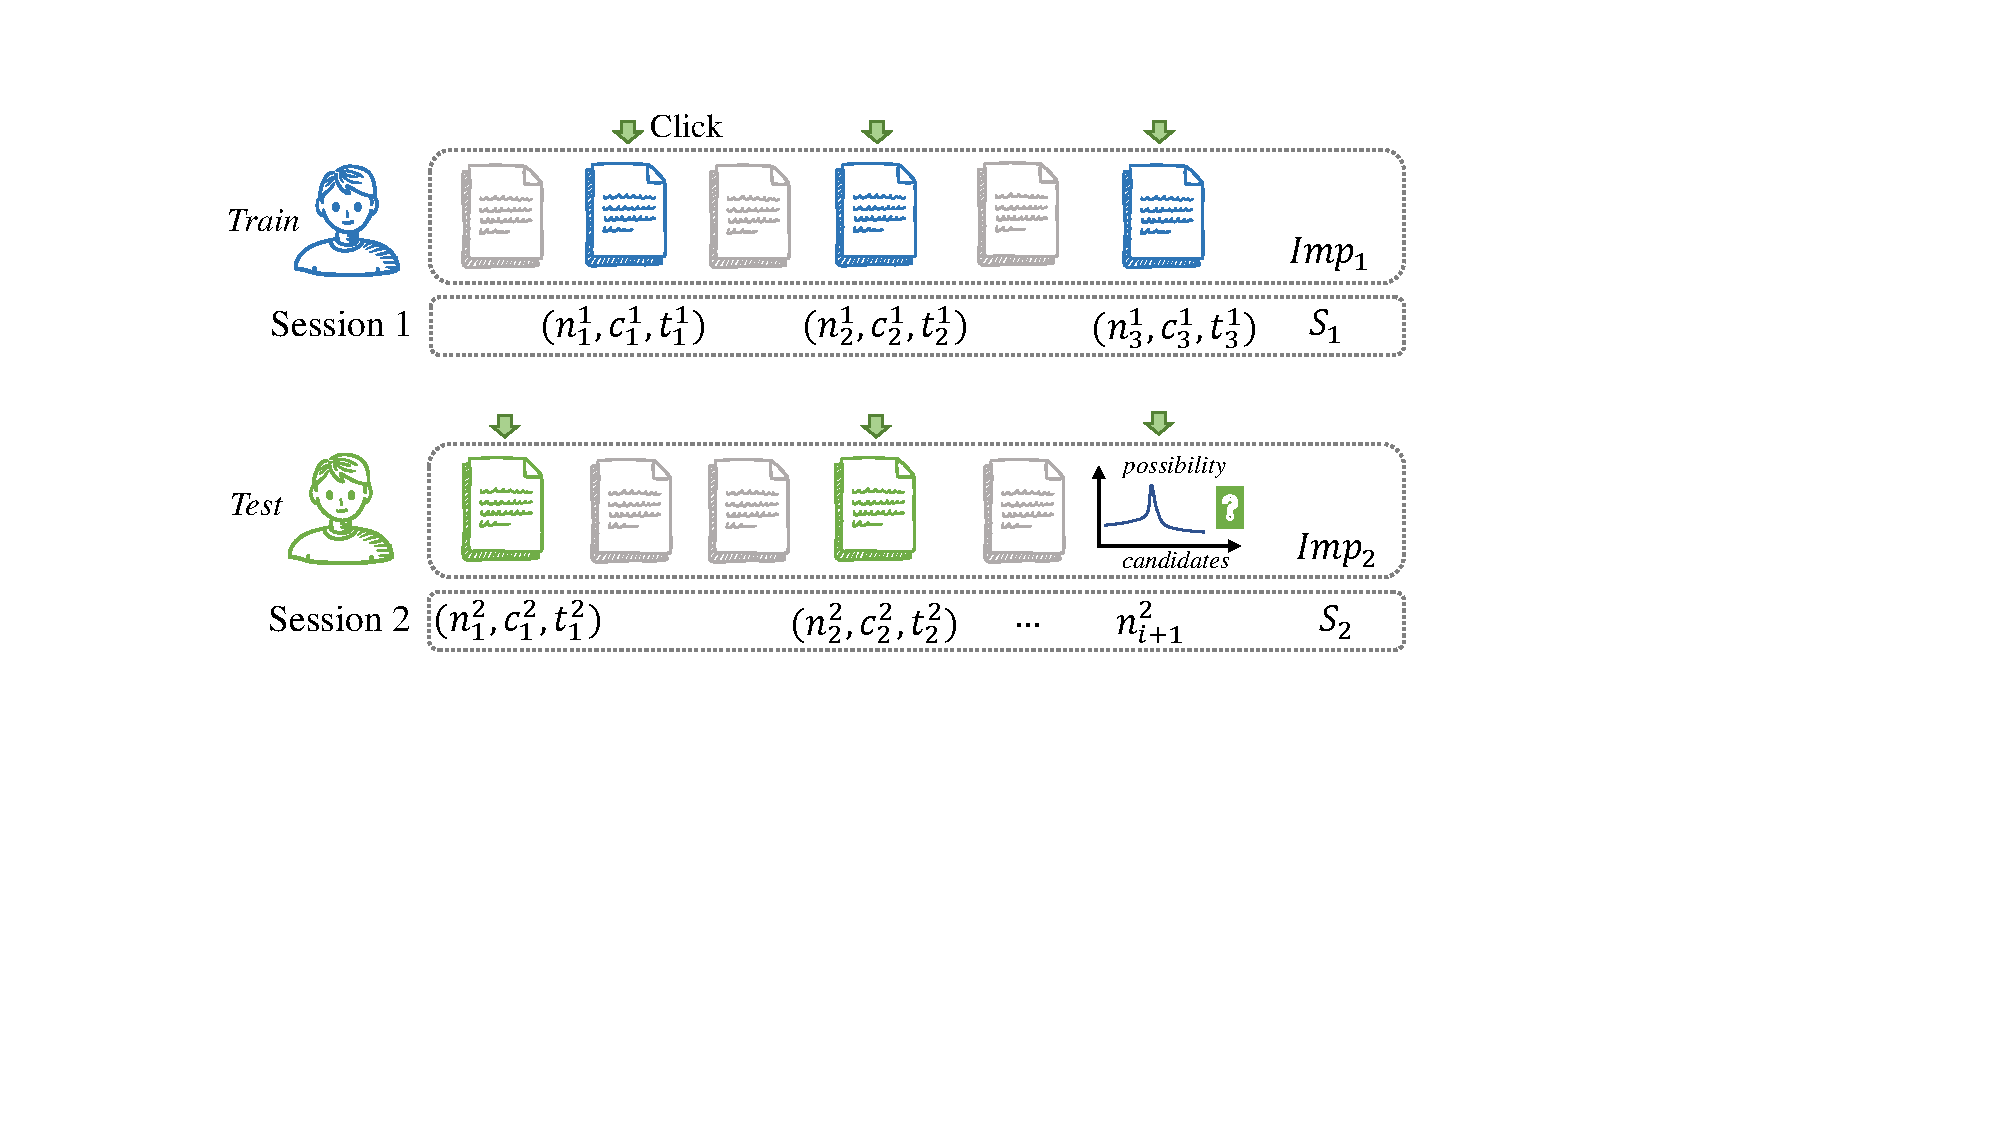
\includegraphics[width=\columnwidth]{fig/task.pdf}
%     \caption{Session-based news recommendation procedure.}
%     \label{fig:task}
% \end{figure}
